\chapter{Background}\label{chap:bkg}

\section{Cell-free systems}
\gls{cfps} systems have existed since the early 1960's as a way to express proteins that are otherwise difficult to express in a living cell~\cite{nirenberg1961dependence}.
These early \gls{cfps} systems were quite crude and had low protein yields, limiting their utility.
More recently, work involving the removal of certain genes~\cite{calhoun2006total} and the improved stability of cofactor regeneration pathways~\cite{jewett2008integrated} has improved the yield of \gls{cfps} systems.

When discussing \gls{cfps} systems, it is important to distinguish between the multiple types of cell-free systems.
One type of cell-free system is created by combining individual purified proteins involved in transcription and translation.
The most widely utilized of these reconstituted cell-free systems is the PURE system~\cite{shimizu2001cell}.
The benefit of these systems is that the system is completely known and controlled.
Since the only things in the system are the proteins that have been deliberately added, users of the systems can be assured that there are no undesirable elements such as nucleases or proteases present.
However, these systems have relatively high costs due to the time and effort required to isolate and purify each of the requisite proteins.

The type of \gls{cfps} system used in this dissertation is an extract-based system created using a crude cell extract.
Creating an extract-based \gls{cfps} system involves growing cells and then lysing them to create a cell extract.
This extract is then used as the basis of the \gls{cfps} system with the assumption that all the important \gls{tx}/\gls{tl} machinery remains intact in the cell extract.
These systems are also known as TXTL systems for this reason.
Growing large quantities of cells is relatively cheap, so these types of systems have the potential to scale more effectively than reconstituted cell-free systems. 
The downside to this method of creating \gls{cfps} systems is that the exact composition of these cell extracts is unknown and can potentially vary between batches of \gls{cfps} systems.
This motivates the need to provide an accurate model of these crude \gls{cfps} systems.

\section{Flux Balance Analysis}
Flux Balance Analysis (\gls{fba}) is one of the most common metabolic modeling tools.
\gls{fba} relies on a mathematical representation of all of the metabolic reactions occurring in an organism.
These reactions are represented using a matrix $S$, a $M \times N$ matrix, where each row represents a separate reaction and each column is a different metabolite.
The entries in this matrix are the stoichiometric coefficient for each metabolite in a given reaction.
Metabolites that are consumed in a reaction are represented using negative numbers.
Flux through each of these reactions can be represented by a vector $v$, which is a 1-dimension vector with a length equal to the number of the reactions.
A crucial assumption in \gls{fba} is that the system is at steady state, so the overall flux through all of the reactions is not changing.
This is expressed mathematically as:
\begin{equation}
S \times v = \vec{0} \\
\end{equation}
where $S$ is the known stoichiometric matrix and $v$ is the unknown flux vector.
The goal of \gls{fba} is to solve for $v$.

This system is underspecified---there are typically more reactions than metabolites ($N >> M$)---so there is no unique solution to this equation.
\gls{fba} solves this issue by specifying an objective function and turning this into an optimization problem.
This objective function can be represented as a vector $c$, whose coefficients select which reactions are to be optimized for.
In the case where the goal of a system is the production of a specific product, $c$ is extremely sparse, having only a single entry.
A common choice of objective function is the Biomass Objective Function, which is a pseudo-reaction that incorporates many essential metabolites necessary for cell growth~\cite{feist2010biomass}.

\gls{fba} also uses a constraint matrix to incorporate biological information into the model.
The constraint matrix specifies constraints on different entries of $v$ in order to limit the amount of flux proceeding through a given reaction.
This allows the model to add in biological information such as reaction irreversibility or metabolite uptake.
For instance, an irreversible reaction is represented by creating a constraint that the lower bound on the flux for that reaction is 0.

Now the \gls{fba} model can be reformulated as a \gls{lp} problem of the form:
\begin{equation}
\centering
\begin{split}
\text{max } Z &= c^Tv \\
&\text{s.t. } S \times v = \vec{0} \\
&\text{and } -\inf < v_0 < \inf \\
&\text{and } 0 < v_1 < \inf \\
&\text{and } 0 < v_2 < 10 \\
...
\end{split}
\end{equation}
where $v_i$ is the flux through reaction $i$ and $Z$ is the flux through the objective function.
$v_0$ is an example of a reversible reaction because flux can go either way.
$v_1$ and $v_2$ are both irreversible reactions, but $v_2$ is constrained due to some external biological knowledge.
\gls{fba} models then use a \gls{lp} solver to find the optimal distribution of fluxes.

\gls{fba} makes a key assumption that the system is at steady state---i.e. the system is stable.
However, \gls{cfps} systems are dynamic systems and do not have a stable period where intake and output are equal until the system is no longer producing protein.
To use \gls{fba} with \gls{cfps}, I consider the period of maximal production of a \gls{cfps} system to be its steady state.
This is the most important interval for a \gls{cfps} system, so \gls{fba} can be used to analyze this pseudo-steady state.

\section{Autoencoders}
Autoencoders are a dimensionality reduction technique with a simple idea: given a dataset, try to reconstruct that dataset by passing it through a lower dimensional subspace.
Deep autoencoders, which I will just refer to as autoencoders, use two neural networks to accomplish this.
One network, called the encoder, performs the mapping from the original dataset to the lower dimensional subspace.
A second network, the decoder, attempts to reconstruct the original dataset by mapping back from the lower dimension back to the dimension of the original dataset.
The original idea behind autoencoders was that this lower dimensional representation of the data served as a compressed version of the data.
Instead of hand designing compression/decompression algorithms, these functions can be learned by a neural network and can therefore be application specific.
In practice, these autoencoders often perform worse than hand-designed compression algorithms.
For instance, autoencoders have difficulty competing with classic algorithms on well-studied problems such as image compression~\cite{theis2017lossy}.
However, autoencoders can also be used as a dimensionality reduction technique.

The lower dimensional subspace that the autoencoders map has been shown to be an effective form of unsupervised dimensionality reduction~\cite{baldi2012autoencoders}.
The transformations that autoencoders learn can sometimes uncover hidden relationships in the data that may be non-obvious in the original dataset.
Biologists often use \gls{pca} to achieve similar goals.
\gls{pca} also projects the data into a subspace, but it does so in a linear manner.
Autoencoders have the advantage that they are able to learn non-linear transformations.

\begin{figure}[t!]
\begin{center}
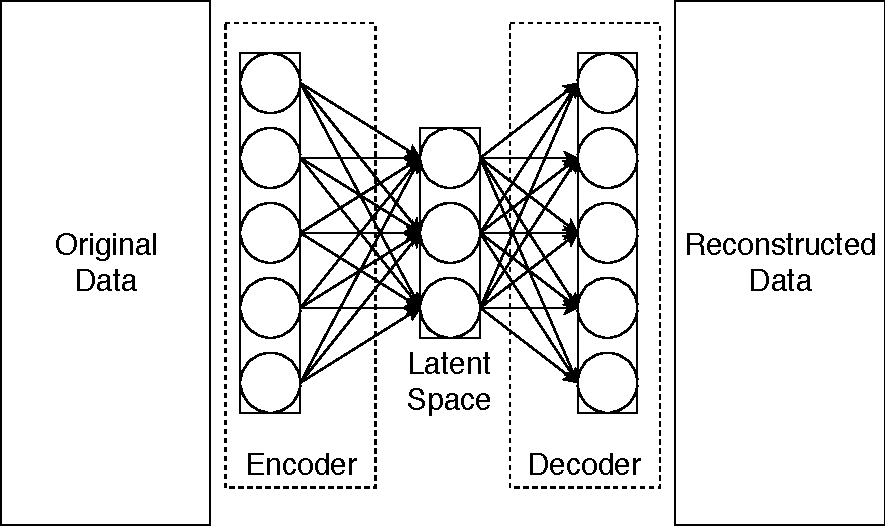
\includegraphics{figs/Autoencoder.pdf}
\caption[Example of a single layer autoencoder]{Example of a single layer autoencoder.
In this case, both the encoder and the decoder are a single layer neural network.
These layers can be stacked to create even more complex dimensionality reductions.}
\end{center}
\label{fig:ae}
\end{figure}

Figure \ref{fig:ae} demonstrates the structure of a very simple autoencoder.
While the main idea of an autoencoder is unchanged, there are a number of different versions of autoencoders that are extensions of this basic idea.
One example is a sparse autoencoder.
In order to force the autoencoder to learn a more general dimensionality reduction, the loss function can include a sparsity constraint to limit the number of activations among the network layers.
This forces the autoencoder to learn a representation with fewer network weights, preventing overfitting.
Another type of autoencoder is a denoising autoencoder.
This type of autoencoder involves taking a noisy representation and mapping it to a clean representation of the data.
These autoencoders add noise to the original data and then try to learn the original representation from the corrupted data.
Despite their differences, almost all of these autoencoder types are trained using reconstruction loss---a measure of how far the autoencoded data is from the original data.

Sometimes it is important to force \glspl{ae} to do more than just learn arbitrary encoding and decoding functions.
For instance, \glspl{vae} are a class of autoencoder that imposes constraints on the encoded representation.
Specifically, \glspl{vae} constrain the encoded representation to be a probability distribution.
So, instead of learning deterministic functions to encode/decode the data, a \gls{vae} learns a mapping to parameters of an encoded probability distribution.
This work uses a normal distribution as the encoded distribution, though other distributions can also be used with \glspl{vae}.
In this case, the encoder learns to map samples to the mean and standard deviation of the normal distribution.
Borrowing terminology from the field of probabilistic models, the encoded dimension is also called the latent space of the \gls{vae}.
In order to decode a data point, \glspl{vae} then samples from the encoded probability distribution to generate a reconstructed data point in the original dimension.

\glspl{vae} measure loss using a combination of two loss terms.
The first part of the error term measures how well the \gls{vae} can reconstruct the original data.
This term is called the reconstruction loss and it measures the distance between the reconstructed data and the original data.
The second loss term acts as a regularizer on the latent space and constrains it to be well formed.
This term is calculated using \gls{kl} divergence, a common way of measuring distance between probability distributions.
For a \gls{vae}, the loss is based on the \gls{kl} divergence between the latent space and a prior distribution, usually the normal distribution. 
With the combination of those two loss terms, the \gls{vae} is then trained the same as any other neural network---by using gradient descent to minimize the loss function.

Define $x_i \in X$ to be the original dataset and $z$ the latent representation learned by the \gls{vae}.
The encoder network can be represented by a function $p$ which has parameters $\theta$.
Similarly, the decoder can be represented as a posterior distribution $q$ that is parameterized by $\phi$.
Then the loss function of a \gls{vae} can therefore be written out as follows:

\begin{equation}\label{eqn:vae-loss}
\mathcal{L}(\theta, \phi) = - E[\log p_{\theta}(x_i | z)] + KL(q_{\phi}(z | x_i) || p(z)) \\
\end{equation}

Minimizing this first part of the loss involves reducing the reconstruction error by maximizing the probability of reconstructing the original data given the latent representation.
Minimizing the second part of the loss requires the latent representation to be similar to the normal distribution.
The \gls{vae} learns the $\theta$ and $\phi$ terms that minimize this function.